\documentclass[bachelor, och, labwork]{shiza}
% параметр - тип обучения - одно из значений:
%    spec     - специальность
%    bachelor - бакалавриат (по умолчанию)
%    master   - магистратура
% параметр - форма обучения - одно из значений:
%    och   - очное (по умолчанию)
%    zaoch - заочное
% параметр - тип работы - одно из значений:
%    referat    - реферат
%    coursework - курсовая работа (по умолчанию)
%    diploma    - дипломная работа
%    pract      - отчет по практике
% параметр - включение шрифта
%    times    - включение шрифта Times New Roman (если установлен)
%               по умолчанию выключен
\usepackage{subfigure}
\usepackage{tikz,pgfplots}
\pgfplotsset{compat=1.5}
\usepackage{float}

%\usepackage{titlesec}
\setcounter{secnumdepth}{4}
%\titleformat{\paragraph}
%{\normalfont\normalsize}{\theparagraph}{1em}{}
%\titlespacing*{\paragraph}
%{35.5pt}{3.25ex plus 1ex minus .2ex}{1.5ex plus .2ex}

\titleformat{\paragraph}[block]
{\hspace{1.25cm}\normalfont}
{\theparagraph}{1ex}{}
\titlespacing{\paragraph}
{0cm}{2ex plus 1ex minus .2ex}{.4ex plus.2ex}

% --------------------------------------------------------------------------%


\usepackage[T2A]{fontenc}
\usepackage[utf8]{inputenc}
\usepackage{graphicx}
\graphicspath{ {./images/} }
\usepackage{tempora}

\usepackage[sort,compress]{cite}
\usepackage{amsmath}
\usepackage{amssymb}
\usepackage{amsthm}
\usepackage{fancyvrb}
\usepackage{listings}
\usepackage{listingsutf8}
\usepackage{longtable}
\usepackage{array}
\usepackage[english,russian]{babel}

\usepackage[colorlinks=false]{hyperref}
\usepackage{url}

\usepackage{underscore}
\usepackage{setspace}
\usepackage{indentfirst} 
\usepackage{mathtools}
\usepackage{amsfonts}
\usepackage{enumitem}
\usepackage{tikz}
\usepackage{minted}

\newcommand{\eqdef}{\stackrel {\rm def}{=}}
\newcommand{\specialcell}[2][c]{%
\begin{tabular}[#1]{@{}c@{}}#2\end{tabular}}

\renewcommand\theFancyVerbLine{\small\arabic{FancyVerbLine}}

\newtheorem{lem}{Лемма}

\begin{document}

% Кафедра (в родительном падеже)
\chair{теоретических основ компьютерной безопасности и криптографии}

% Тема работы
\title{Цепные дроби и квадратные сравнения}

% Курс
\course{5}

% Группа
\group{531}

% Факультет (в родительном падеже) (по умолчанию "факультета КНиИТ")
\department{факультета КНиИТ}

% Специальность/направление код - наименование
%\napravlenie{09.03.04 "--- Программная инженерия}
%\napravlenie{010500 "--- Математическое обеспечение и администрирование информационных систем}
%\napravlenie{230100 "--- Информатика и вычислительная техника}
%\napravlenie{231000 "--- Программная инженерия}
\napravlenie{100501 "--- Компьютерная безопасность}

% Для студентки. Для работы студента следующая команда не нужна.
% \studenttitle{Студентки}

% Фамилия, имя, отчество в родительном падеже
\author{Улитина Ивана Владимировича}

% Заведующий кафедрой
% \chtitle{} % степень, звание
% \chname{}

%Научный руководитель (для реферата преподаватель проверяющий работу)
\satitle{профессор} %должность, степень, звание
\saname{В. А. Молчанов}

% Руководитель практики от организации (только для практики,
% для остальных типов работ не используется)
% \patitle{к.ф.-м.н.}
% \paname{С.~В.~Миронов}

% Семестр (только для практики, для остальных
% типов работ не используется)
%\term{8}

% Наименование практики (только для практики, для остальных
% типов работ не используется)
%\practtype{преддипломная}

% Продолжительность практики (количество недель) (только для практики,
% для остальных типов работ не используется)
%\duration{4}

% Даты начала и окончания практики (только для практики, для остальных
% типов работ не используется)
%\practStart{30.04.2019}
%\practFinish{27.05.2019}

% Год выполнения отчета
\date{2023}

\maketitle

% Включение нумерации рисунков, формул и таблиц по разделам
% (по умолчанию - нумерация сквозная)
% (допускается оба вида нумерации)
% \secNumbering

%-------------------------------------------------------------------------------------------

\section{Постановка задачи}

    \textbf{Цель работы} - изучение основных свойств цепных дробей и квадратных
    сравнений. 

    Порядок выполнения работы:
    \begin{enumerate}
        \item Разобрать алгоритм разложения чисел в цепную дробь и привести его
        программную реализацию;
        \item Разобрать алгоритмы приложений цепных дробей и привести их
        программную реализацию;
        \item Разобрать алгоритмы вычисления символов Лежандра и Якоби и
        привести их программную реализацию;
        \item Рассмотреть алгоритмы извлечения квадратного корня в кольце
        вычетов.
    \end{enumerate}

\section{Теоретические сведения}

    \subsection{Цепные дроби}

        Рассмотрим рациональное число $r$, представленное в виде несократимой
        дроби $r = \frac{a_0}{a_1}$. Так как НОД$(a_0, a_1) = 1$, то результат
        вычисления этого наибольшего общего делителя по алгоритму Евклида имеет
        вид

        $$a_0 = a_1 q_1 + a_2, 0 \leq a_2 < a_1,$$
        $$a_1 = a_2 q_2 + a_3, 0 \leq a_3 < a_2,$$
        $$\cdots$$
        $$a_{k-2} = a_{k-1} q_{k-1} + a_{k}, 0 \leq a_{k} < a_{k-1},$$
        $$a_{k-1} = a_k q_k, \text{где } a_k = \text{НОД} (a_0, a_1) = 1.$$

        Эти равенства можно переписать в виде:

        $$\frac{a_0}{a_1} = q_1 + \frac{a_2}{a_1}, \frac{a_1}{a_2} = q_2 +
        \frac{a_3}{a_2}, \dots, \frac{a_{k-2}}{a_{k-1}} = q_{k-1} +
        \frac{a_k}{a_{k-1}} = q_{k-1} + \frac{1}{q_k}.$$

        Тогда рациональное число $r$ можно представить следующим образом:

        $$r = \frac{a_0}{a_1} = q_1 + \frac{a_2}{a_1} = q_1 + \frac{1}{\frac{a_1}{a_2}} = \dots = q_1 + \frac{1}{q_2 + \frac{1}{\ddots + \frac{1}{q_{k-1} + \frac{1}{q_k}}}},$$

        где $q_1$ "--- целое число и $q_2, \dots, q_k$ "--- целые положительные
        числа.

        \textbf{Определение:} Выражение вида 

        $$q_1 + \frac{1}{q_2 + \frac{1}{\ddots + \frac{1}{q_{k-1} +
        \frac{1}{q_k}}}}$$

        принято называть цепной (или непрерывной) дробью с неполными частными
        $q_1, q_2, \dots, q_k$ и обозначать символом $(q_1 ; q_2, \dots, q_k).$

        Таким образом, любая несократимая рациональная дробь $\frac{a_0}{a_1}$
        может быть представлена в виде цепной дроби $\frac{a_0}{a_1} = (q_1 ;
        q_2, \dots, q_k)$ с неполными частными $q_1, q_2, \dots, q_k$,
        полученными в результате вычисления по алгоритму Евклида наибольшего
        общего делителя взаимно простых чисел $a_0, a_1$.

    \subsection{Подходящие дроби и их свойства}

        Для цепной дроби $\frac{a_0}{a_1} = (q_1 ; q_2, \dots, q_k)$ выражения
        $\delta_1 = q_1$, $\delta_2 = q_1 + \frac{1}{q_2}$, $\dots$, $\delta_k =
        q_1 + \frac{1}{q_2 + \frac{1}{\ddots + \frac{1}{q_{k-1} +
        \frac{1}{q_k}}}}$ называются подходящими дробями конечной цепной дроби
        $(q_1 ; q_2, \dots, q_k)$ и обозначаются символами $\delta_i = (q_1 ;
        q_2, \dots, q_i)$, где $1 \leq i \leq k$.

        Аналогично определяются подходящие дроби $\delta_i = (q_1 ; q_2, \dots,
        q_i)$ для бесконечной цепной дроби $(q_1 ; q_2, \dots, q_k, \dots)$.

        Индукцией по номеру $i = \overline{1,k}$ можно доказать следующие важные
        свойства таких подходящих дробей:

        \begin{enumerate}
            \item каждая подходящая дробь $\delta_i$ $(i = \overline{1, k})$
            является несократимой рациональной дробью $\delta_i =
            \frac{P_i}{Q_i}$ с числителем $P_i$ и знаменателем $Q_i$, которые
            вычисляются по следующим рекуррентным формулам:

            $$P_i = q_i P_{i-1} + P_{i-2}, Q_i = q_i Q_{i-1} + Q_{i-2}$$

            с начальными условиями $P_{-1} = 0, P_{0} = 1, Q_{-1} = 1, Q_{0} =
            0$;

            \item числители и знаменатели двух последовательных подходящих
            дробей удовлетворяют равенству $P_i Q_{i-1} - P_{i-1} Q_i = (-1)^i$
            для всех $i = \overline{1, k}$;

            \item $P_i$, $Q_i$ взаимно просты;
            \item $$\frac{P_i}{Q_i} - \frac{P_{i-1}}{Q_{i-1}} = \frac{(-1)^i}{Q_i Q_{i-1}};$$
            \item $$\delta_{2n} > \delta_{2n-1};$$
            \item $$P_i Q_{i-2} - P_{i-2} Q_i = q_i \cdot (-1)^{i-1};$$
            \item $$\frac{P_i}{Q_i} - \frac{P_{i-2}}{Q_{i-2}} = \frac{q_i \cdot (-1)^{i-1}}{Q_i Q_{i-2}};$$
            \item $$\delta_{2n} = \frac{P_{2n}}{Q_{2n}} \text{"--- убывающая последовательность},$$
            
            $$\delta_{2n-1} = \frac{P_{2n-1}}{Q_{2n-1}} \text{"--- возрастающая последовательность},$$

            $$\delta_1 < \delta_3 < \dots < \delta_{2n - 1} < \dots \leq \frac{a}{b} \leq \dots < \delta_{2n} < \dots < \delta_4 < \delta_2;$$

            \item $$\frac{P_n}{Q_n} = q_1 + \sum_{i=1}^{n} \frac{(-1)^i}{Q_i Q_{i-1}} \text{ (сходится по признаку Лейбница)};$$
            \item $$Q_n = q_n \cdot Q_{n-1} + Q_{n-2} \geq Q_{n-1} + Q_{n-2} \geq 2 Q_{n-2} \geq 2^{\frac{n - 2}{2}}$$
            \item $$|\alpha - \delta_i| \leq |\delta_i - \delta_{i - 1}| = \frac{1}{Q_i Q_{i-1}}.$$
            \item Если все $q_i > 0$, то $\lim_{n \to \infty} \delta_n =
            \alpha;$ в частности, любое число $\alpha \in \mathbf{R}_+$
            представляется цепной дробью.

        \end{enumerate}

    \subsection{Приложения цепных дробей}
    
        В качестве приложений цепных дробей выделяют:

        \begin{enumerate}
            \item Решение линейных диофантовых уравнений $ax + by = c$.
            \item Вычисление обратных элементов в кольце вычетов $\mathbb{Z}_m$.
            \item Решение линейных сравнений $ax \equiv b \pmod m$.
        \end{enumerate}

        \subsubsection{Диофантовые уравнения}

            \textbf{Определение:} Диофантовыми уравнениями называются алгебраические
            уравнения с целочисленными коэффициентами, решение которых отыскивается
            в целых числах.

            Например, диофантовым уравнением является уравнение вида $$ax - by = 1$$
            с целыми неотрицательными коэффициентами $a, b$. Если коэффициенты $a,
            b$ удовлетворяют условию НОД$(a, b) = 1$ и $\frac{P_{k-1}}{Q_{k-1}}$
            "--- предпоследняя подходящая дробь представления числа $\frac{a}{b}$ в
            виде цепной дроби, то из равенств $P_{k}Q_{k-1} - P_{k-1}Q_{k} =
            (-1)^k,$ $\frac{a}{b} = \delta_k = \frac{P_k}{Q_k}$ следует, что

            $$a (-1)^k Q_{k-1} - b (-1)^k P_{k-1} = 1,$$

            т.е. значения $x = (-1)^k Q_{k-1}, y = (-1)^k P_{k-1}$ являются
            целочисленными решениями уравнения $ax - by = 1$. Легко видеть, что все
            целые решения исходного диофантова уравнения $ax - by = 1$ находятся по
            формулам:
            
            $$x = (-1)^k Q_{k-1} + bt, y = (-1)^k P_{k-1} + at,$$

            где $t$ "--- произвольное целое число.

            Нетрудно убедиться, что все решения диофантова уравнения $ax - by = c$ с
            взаимно простыми коэффициентами $a, b$ находятся по формулам:

            $$x = (-1)^k c Q_{k-1} + bt, y = (-1)^k c P_{k-1} + at,$$

            где $t$ "--- произвольное целое число.

        \subsubsection{Вычисление обратных элементов}

            \textbf{Определение:} Обратным элементом к числу $a$ по модулю $m$
            называется такое число $b$, что $ab \equiv 1 \pmod m$. Обратный
            элемент обозначают как $a^{-1}$.

            Для нуля обратного элемента не существует никогда, для остальных же
            элементов обратный элемент может как существовать, так и нет.
            Утверждается, что обратный элемент существует только для тех
            элементов $a$, которые взаимно просты с модулем $m$.

            Для нахождения обратного элемента по модулю можно использовать
            расширенный алгоритм Евклида. Чтобы показать это, можно рассмотреть
            следующее уравнение:

            $$ax + my = 1.$$

            Это уравнение является линейным диофантовым уравнением с двумя
            переменными. Посколько единица может делиться только на единицу, то
            уравнение имеет решение только если НОД$(a, m) = 1$.

            Как уже ранее утверждалось, решение можно найти с помощью
            расширенного алгоритма Евклида. При этом, если мы возьмём от обеих
            частей уравнения остаток по модулю $m$, то получим:

            $$ax = 1 \pmod m,$$

            откуда видно, что найденное $x$ является обратным элементом к $a$.

        \subsubsection{Решение линейных сравнений}

            Сравнение двух целых чисел по модулю натурального числа $m$ "---
            математическая операция, позволяющая ответить на вопрос о том, дают
            ли два выбранных целых числа при делении на m один и тот же остаток.

            Сравнимость чисел $a$ и $b$ по модулю сравнения $m$ записывается
            как:

            $$a \equiv b \pmod m.$$

            \textbf{Определение:} Выражение

            $$a \cdot x \equiv b \pmod m$$

            называется сравнением первой степени или линейным сравнением по
            модулю $m$.
            
            Для проверки существования решений сравнения сначала вычисляется
            НОД$(a, m)$. Если $b$ не кратно полученному НОД, то у сравнения нет
            решений. Если кратно, то количество решений по модулю $m$ равно
            полученному НОД.

            Существует несколько алгоритмов нахождения всех решений сравнения,
            но в рамках рассмотрения приложений цепных дробей применяется
            алгоритм решения линейных диофантовых уравнений с двумя переменными.
            В самом деле, сравнение эквивалентно следующему линейному
            диофантовому уравнению:

            $$a \cdot x + m \cdot y = b \pmod m,$$

            исходя из которого можно получить общую формулу решения, после чего
            выбрать все частные решения в диапазоне от 0 до $m$.

    \subsection{Алгоритмы вычисления символов Лежандра и Якоби}
    
        Пусть $p > 2$ "--- простое число.

        \textbf{Определение:} Число $a \in \mathbb{Z}_p$ называется квадратичным
        вычетом по модулю $p$, если 

        $$(\exists x \in \mathbb{Z}) \text{ } x^2 \equiv a \pmod p.$$

        В противном случае число $a$ называется квадратичным невычетом по модулю
        $p$.

        \textbf{Определение:} Для нечетного простого числа $p$ символом Лежандра
        числа $a \in \mathbb{Z}$ называется выражение

        \[\left(\frac{a}{p}\right) =
            \begin{cases}
                1 & \quad \text{если } a \text{ "--- квадратичный вычет по модулю } p\\
                -1 & \quad \text{если } a \text{ "--- квадратичный невычет по модулю } p\\
                0 & \quad \text{если } a \equiv 0 \pmod p.
            \end{cases}
        \]

        \textbf{Свойства символа Лежандра:}

        \begin{enumerate}
            \item $a \equiv b \pmod p \Longrightarrow  \left(\frac{a}{p}\right) = \left(\frac{b}{p}\right),$
            \item $\left(\frac{ac^2}{p}\right) = \left(\frac{a}{p}\right)$ для любого $c \in \mathbb{Z}$, НОД$(c, p) = 1.$
            \item Критерий Эйлера $\left(\frac{a}{p}\right) = a^{\frac{p - 1}{2}} \pmod p$ для НОД$(a, p) = 1.$
            \item $\left(\frac{ab}{p}\right) = \left(\frac{a}{p}\right) \cdot \left(\frac{b}{p}\right)$,
            \item \[\left(\frac{1}{p}\right) = 1, \left(\frac{-1}{p}\right) = (-1)^{\frac{p-1}{2}} = 
            \begin{cases}
                1 & \quad \text{если } p \equiv 1 \pmod 4,\\
                -1 & \quad \text{если } p \equiv 3 \pmod 4.
            \end{cases}\]
            \item \[\left(\frac{2}{p}\right) = (-1)^{\frac{p^2 - 1}{8}} = 
            \begin{cases}
                1 & \quad \text{если } p \equiv \pm 1 \pmod 8,\\
                -1 & \quad \text{если } p \equiv \pm 3 \pmod 8.
            \end{cases}\]
            \item Квадратичный закон взаимности Гаусса:
            $$\left(\frac{p}{q}\right) = \left(\frac{q}{p}\right) \cdot
            (-1)^{\frac{p-1}{2} \cdot \frac{q-1}{2}}$$ для любых нечетных
            простых чисел $p, q.$
        \end{enumerate}

        \textbf{Определение:}
        
        Пусть натуральное число $n = p_1^{\alpha_1} \cdot \dots \cdot
        p_k^{\alpha_k}.$ Символом Якоби числа $a \in \mathbb{Z}$ называется
        выражение $$\left(\frac{a}{n}\right) =
        \left(\frac{a}{p_1}\right)^{\alpha_1} \cdot \dots \cdot
        \left(\frac{a}{p_k}\right)^{\alpha_k}.$$

        Символ Якоби для простого числа $n$ совпадает с символом Лежандра и
        удовлетворяет почти всем свойствам символа Лежандра (хотя в общем случае
        символ Якоби не связан с квадратичными вычетами).

        Символ Якоби позволяет упростить вычисление символа Лежандра
        $\left(\frac{a}{p}\right)$ (без разложения числа на множители).



\section{Результаты работы}

    \subsection{Описание алгоритма разложения чисел в цепную дробь и алгоритмов
    приложений цепных дробей}

        \underline{Алгоритм 1 - алгоритм разложения чисел в цепную дробь}\\
            \textit{Вход}: целые числа $a, b$.\\
            \textit{Выход}: массив $r$ из чисел $r_1, r_2, \dots, r_k$ "--- цепная дробь.\\
            \underline{Шаг 1.} Создать пустой массив $r$.\\
            \underline{Шаг 2.} Взять целую часть от деления $a$ на $b$ и добавить в массив.\\
            \underline{Шаг 3.} Определить $c = a$. После этого переопределить $a
            = b$, $b = c \% b$ (то есть остаток от деления $c$ на $b$).\\
            \underline{Шаг 4.} Если $b$ не равно нулю, перейти к шагу $2$, иначе
            к шагу $5$.\\
            \underline{Шаг 5.} Результат: массив $r = r_1, \dots, r_k$, который
            представляет собой разложение чисел в цепную дробь.\\
            
        \underline{Псевдокод:}
            \begin{minted}[breaklines,fontsize=\small]{text}
            функция Непрерывная_дробь(a, b):
            дробь = пустой_список
            
            пока b не равно 0:
                дробь.добавить(целая_часть(a / b))
                c = a
                a = b
                b = c % b
            
            вернуть дробь                  
            \end{minted}

            Трудоемкость алгоритма $O(\log(\max\{a, b\}))$.\\

        \underline{Алгоритм 2 - алгоритм решения линейных диофантовых уравнений}\\
            \textit{Вход}: целые числа $a, b, c$ "--- коэффициенты уравнения.\\
            \textit{Выход}: целые числа $x, y$ "--- решение уравнения вида $ax - by = c$.\\
            \underline{Шаг 1.} Определить массив $r$ "--- разложение чисел $a, b$ в
            цепную дробь с помощью алгоритма $1$.\\ 
            \underline{Шаг 2.} Определить массивы $p = \{0, 1\}$ и $p = \{1, 0\}$.\\
            \underline{Шаг 3.} Положить $i = 2$.\\
            \underline{Шаг 4.} Пусть $c = r_{i - 2}$. Добавить в массив $p$
            значение $p_{i-1} \cdot c + p_{i-2}$. Добавить в массив $q$
            значение $q_{i-1} \cdot c + q_{i-2}$.\\
            \underline{Шаг 5.} Пусть $k$ "--- длина массива $r$. Если $i < k +
            2$, то $i = i + 1$ и перейти к шагу $4$. Иначе перейти к шагу $6$.\\
            \underline{Шаг 6.} Определить $x = q_{k-1} \cdot (-1)^k \cdot c + bt$, $y =
            p_{k-1} \cdot (-1)^k \cdot c + at$.\\
            \underline{Шаг 7.} Результат: $x, y$.\\
            
        \underline{Псевдокод:}
            \begin{minted}[breaklines,fontsize=\small]{text}
            функция Диофантово_уравнение(a, b, c):
            дробь = Непрерывная_дробь(a, b)
            p = [0, 1]
            q = [1, 0]
            
            для i от 2 до длина(дробь) + 2:
                коэф = дробь[i - 2]
                p.добавить(p[i - 1] * коэф + p[i - 2])
                q.добавить(q[i - 1] * коэф + q[i - 2])
        
            k = длина(дробь)
            x = q[k] * степень(-1, k) * c
            y = p[k] * степень(-1, k) * c
        
            вернуть (x, y, a, b)
                         
            \end{minted}

            Трудоемкость алгоритма $O(k)$, где $k$ "--- количество элементов в
            разложении чисел $a, b$ на непрерывную дробь.\\


        \underline{Алгоритм 3 - алгоритм вычисления обратных элементов в кольце вычетов}\\
            \textit{Вход}: целые число $a$ и модуль $m$.\\
            \textit{Выход}: $r$ "--- обратный элемент числа $a$ в кольце вычетов $\mathbb{Z}_m$.\\
            \underline{Шаг 1.} Положить $b_1 = 1$.\\ 
            \underline{Шаг 2.} С помощью расширенного алгоритма Евклида от $a$ и
            $m$ получить значения $d, p, q$ "--- НОД и коэффициенты перед
            большим и меньшим числом соответственно.\\
            \underline{Шаг 3.} Определить $b_2 = \frac{b}{d}$, $n = \frac{m}{d}$, $k = 1$.\\
            \underline{Шаг 4.} Если остаток от деления $d - 1$ на $2$ не равен
            $0$, то $k = k - 1$.\\
            \underline{Шаг 5.} Определить $r = k \cdot p \cdot b_2 \pmod n$.\\
            \underline{Шаг 6.} Результат: $r$.\\

        \underline{Псевдокод:}
            \begin{minted}[breaklines,fontsize=\small]{text}
            функция Получить_обратный_элемент(a, m):
            b = 1
            (_, d, p, q) = Расширенный_алгоритм_Евклида(a, m, 0, 0)
            новый_b = b / d
            новый_m = m / d
            k = 1
            если (d - 1) % 2 != 0 то:
                k = -1
            
            ответ = ((k * p * новый_b) % новый_m).остаток_по_модулю(m)
        
            вернуть ответ
            \end{minted}

            Трудоемкость алгоритма $O(\log(m)^2)$.\\


        \underline{Алгоритм 4 - алгоритм решения линейных сравнений $ax \equiv b \pmod m$}\\
            \textit{Вход}: целые числа $a, b, m$.\\
            \textit{Выход}: массив $s = \{s_1, s_2, \dots, s_k\}$, содержащий
            решения линейных сравнений $1$-й степени.\\
            \underline{Шаг 1.} С помощью расширенного алгоритма Евклида от $a$ и
            $m$ получить значения $d, p, q$ "--- НОД и коэффициенты перед
            большим и меньшим числом соответственно.\\
            \underline{Шаг 2.} Определить $b_2 = \frac{b}{d}$, $n = \frac{m}{d}$, $k = 1$.\\
            \underline{Шаг 3.} Если остаток от деления $d - 1$ на $2$ не равен
            $0$, то $k = k - 1$. \\
            \underline{Шаг 4.} Определить $s_1 = k \cdot p \cdot b_2 \pmod n$.
            Определить массив $s$ и добавить в него $s_1$.\\
            \underline{Шаг 5.} Определить $i = 1$.\\
            \underline{Шаг 6.} Опредилить $s_{i+1} = s_1 + n \cdot i \pmod m$ и
            добавить его в массив $s$.\\
            \underline{Шаг 7.} Если $i < d$, то $i = i + 1$ и перейти к шагу
            $6$, иначе перейти к шагу $8$.\\
            \underline{Шаг 8.} Результат: массив $s$.\\

        \underline{Псевдокод:}
            \begin{minted}[breaklines,fontsize=\small]{text}
            функция Решение_линейного_сравнения(a, b, m):
                (_, d, p, q) = Расширенный_алгоритм_Евклида(a, m, 0, 0)

                новый_b = b / d
                новый_m = m / d

                k = 1
                если (d - 1) % 2 != 0 то:
                    k = -1

                первый_ответ = ((k * p * новый_b) % новый_m).остаток_по_модулю(m)
                решения = [первый_ответ]

                для i от 1 до d:
                    решения.добавить((решения[0] + новый_m * i).остаток_по_модулю(m))

                вывести_массив(решения)
            \end{minted}

            Трудоемкость алгоритма $O(\log(\max\{a, m\}))$.\\


    \subsection{Описание алгоритмов вычисления символов Лежандра и Якоби и
    алгоритма извлечения квадратного корня в кольце вычетов}

        \underline{Алгоритм 5 - алгоритм вычисления символа Лежандра}\\
            \textit{Вход}: целые числа $a, p$.\\
            \textit{Выход}: целое число, равное значению символа Лежандра
            $\left(\frac{a}{p}\right)$.\\
            \underline{Шаг 1.} Если $a < 0$, то по свойству $4$ выделить
            множитель $\left(\frac{-1}{p}\right)$.\\
            \underline{Шаг 2.} Замена $a$ на остаток от деления на $p$.\\
            \underline{Шаг 3.} Представить $a = p_1^{\alpha_1} \cdot \dots \cdot
            p_k^{\alpha_k}$ и вычислить по свойству $4$
            $$\left(\frac{a}{p}\right) = \left(\frac{p_1}{p}\right)^{\alpha_1}
            \cdot \dots \cdot \left(\frac{p_k}{p}\right)^{\alpha_k}.$$ Множители
            с четными степенями $\alpha_i$ опускаются, а вместо множителей
            $\left(\frac{p_i}{p}\right)^{\alpha_i}$ с нечетными степенями
            $\alpha_i$ оставить $\left(\frac{p_i}{p}\right)$.\\
            \underline{Шаг 4.} Если $p_i = 2$, то вычислить согласно свойству
            $6$: $\left(\frac{2}{p}\right) = (-1)^{\frac{p^2 - 1}{8}}$.\\
            \underline{Шаг 5.} К остальным символам $\left(\frac{p_i}{p}\right)$
            применяется квадратичный закон Гаусса.\\
            \underline{Шаг 6.} Если $a$ не равно нулю "--- вернуться к шагу
            $2$. Иначе перейти к шагу $7$.\\
            \underline{Шаг 7.} Результат: целое число, равное значению символа
            Лежандра $\left(\frac{a}{p}\right)$.\\

            \underline{Псевдокод:}
            \begin{minted}[breaklines,fontsize=\small]{text}
            функция Символ_Лежандра(a, p):
            если Является_простым(p) то:
                вернуть Символ_Якоби(a, p)
        
            a = a % p
            если a < 0 то:
                a = a + p
        
            результат = 1
            пока a не равно 0:
                пока a делится на 2:
                    a = a / 2
                    если p % 8 равно 3 или p % 8 равно 5 то:
                        результат = -результат
        
                обменять_местами(a, p)
        
                если a % 4 равно 3 и p % 4 равно 3 то:
                    результат = -результат
        
                a = a % p
        
            если p равно 1 то:
                вернуть результат
            иначе:
                вернуть 0
        
            \end{minted}

            Трудоемкость алгоритма $O(\log(a) \cdot \log(p))$.\\

        \underline{Алгоритм 6 - алгоритм вычисления символа Якоби}\\
            \textit{Вход}: целые числа $a, p$.\\
            \textit{Выход}: целое число, равное значению символа Якоби
            $\left(\frac{a}{p}\right)$.\\
            \underline{Шаг 1.} Заменить $a$ на такое $b$, что $a \equiv b \pmod
            p$ и $|b| < \frac{p}{2}$.\\
            \underline{Шаг 2.} Если $b < 0$, то по свойству $4$ выделить
            множитель $\left(\frac{-1}{p}\right)$.\\
            \underline{Шаг 3.} Если $b$ "--- четное, то представить $b = 2^t
            \cdot a_1$ и при нечетном $t$ вычислить $\left(\frac{2}{p}\right) =
            (-1)^{\frac{p^2 - 1}{8}}$.\\
            \underline{Шаг 4.} К символу $\left(\frac{a_1}{p}\right)$
            применяется квадратичный закон взаимности Гаусса.\\
            \underline{Шаг 5.} При необходимости перейти к шагу $1$. Иначе
            перейти к шагу $6$.\\
            \underline{Шаг 6.} Результат: целое число, равное значению символа
            Якоби $\left(\frac{a}{p}\right)$.\\

            \underline{Псевдокод:}
            \begin{minted}[breaklines,fontsize=\small]{text}
            функция Символ_Якоби(a, n):
            t = 1
            пока a не равно 0:
                пока a делится на 2:
                    a = a / 2
                    n_mod_8 = n % 8
                    если n_mod_8 равно 3 или n_mod_8 равно 5 то:
                        t = -t
        
                обменять_местами(a, n)
                если a % 4 равно 3 и n % 4 равно 3 то:
                    t = -t
        
                a = a % n
        
            если n равно 1 то:
                вернуть t
            иначе:
                вернуть 0
            \end{minted}


            Трудоемкость алгоритма $O(\log(p))$.\\

        \underline{Алгоритм 7 - алгоритм извлечения квадратного корня в кольце вычетов}\\
            \textit{Вход}: Число $a$ и модуль $p$ (где $p - 1 = 2^m q$).\\
            \textit{Выход}: Число $x$ "--- квадратный корень числа $a$ в кольце
            вычетов $\mathbb{Z}_m$.\\
            \underline{Шаг 1.} Случайным образом выбрать такое $b$, что
            $\left(\frac{b}{p}\right) = -1$.\\
            \underline{Шаг 2.} Вычислить последовательность $a_1, \dots, a_n$
            элементов поля $\mathbb{Z}_p$ и последовательность чисел $k_1,
            \dots, k_n$ по правилу:
            \begin{enumerate}
                \item $a_1 = a,$ $a_{i+1} = a_i \cdot b^{2^{m - k_i}} \pmod p,$ $i \geq 1;$
                \item $k_i$ "--- наименьшее $k \geq 0,$ при котором $a_i^{2^k q} \equiv 1 \pmod p$ 
            \end{enumerate}
            \underline{Шаг 3.} Если равенство $k_n = 0$ не выполняется, перейти
            к шагу $2$.\\
            \underline{Шаг 4.} Вычислить последовательность элементов $r_n,
            \dots, r_1$ элементов поля $\mathbb{Z}_p$ по правилу:
            
            $$r_n = a_n^{\frac{q + 1}{2}} \pmod p, \text{ } r_i = r_{i +
            1}(b^{2^{{m - k_i - 1}}})^{-1} \pmod p, \text{ } i \geq 1.$$\\
            \underline{Шаг 5.} Положить $x = r_1$ "--- искомое решение.\\
            \underline{Шаг 6.} Результат: число $x$ "--- квадратный корень
            числа $a$ в кольце вычетов $\mathbb{Z}_m$.

            \underline{Псевдокод:}
            \begin{minted}[breaklines,fontsize=\small]{text}
            функция Квадратный_корень_в_кольце_вычетов(a, p):
            если символ_Лежандра(a, p) не равно 1 то:
                вернуть -1
        
            q = p - 1
            s = 0
        
            пока q делится на 2:
                q = q / 2
                s = s + 1
        
            если s равно 1 то:
                x = a.в_степень((p + 1) / 4) % p
                вернуть x
        
            z = 2
        
            пока символ_Лежандра(z, p) не равно -1:
                z = z + 1
        
            c = z.в_степень(q) % p
            r = a.в_степень((q + 1) / 2) % p
            t = a.в_степень(q) % p
            m = s
        
            пока t не равно 1:
                i = 0
                zz = t
        
                пока zz не равно 1:
                    zz = (zz * zz) % p
                    i = i + 1
        
                b = c.в_степень(2 в степени (m - i - 1)) % p
                r = (r * b) % p
                t = (t * b.в_степень(2)) % p
                c = b.в_степень(2) % p
                m = i
        
            вернуть r
            \end{minted}

            Трудоемкость алгоритма $O(\log(p)^4)$\\
    
    \subsection{Код программы, реализующей рассмотренные алгоритмы}

        \inputminted[breaklines,fontsize=\small,linenos]{rust}{../code/src/main.rs}

    \subsection{Результаты тестирования программ}
        \begin{figure}[H]
            \centering
            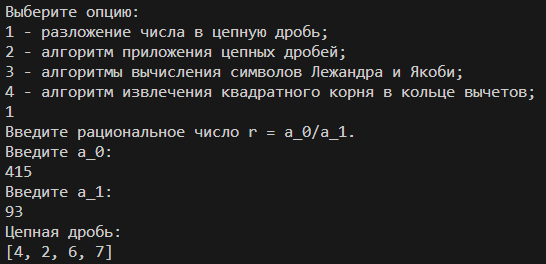
\includegraphics[width=0.8\textwidth]{pic/1.png}
            \caption{Тест алгоритма разложения в цепную дробь}
        \end{figure}

        \begin{figure}[H]
            \centering
            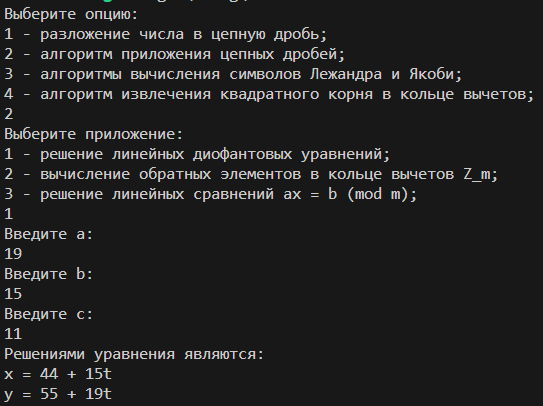
\includegraphics[width=0.8\textwidth]{pic/2.png}
            \caption{Тест приложения цепной дроби, решения линейных диофантовых уравнений}
        \end{figure}

        \begin{figure}[H]
            \centering
            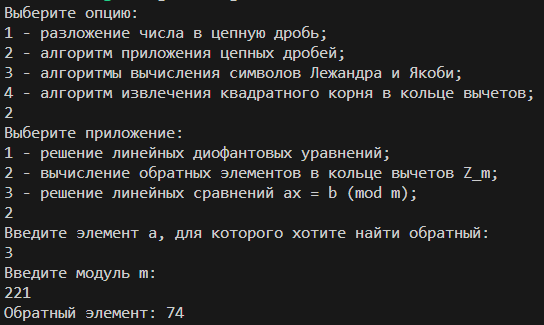
\includegraphics[width=0.8\textwidth]{pic/3.png}
            \caption{Тест приложения цепной дроби, вычисления обратных элементов в кольце вычетов}
        \end{figure}

        \begin{figure}[H]
            \centering
            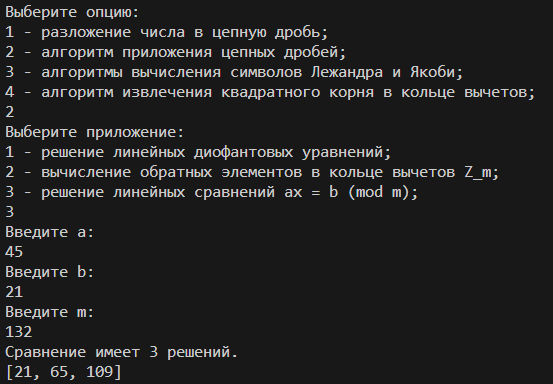
\includegraphics[width=0.8\textwidth]{pic/4.png}
            \caption{Тест приложения цепной дроби, решения линейных сравнений 1-ой степени}
        \end{figure}

        \begin{figure}[H]
            \centering
            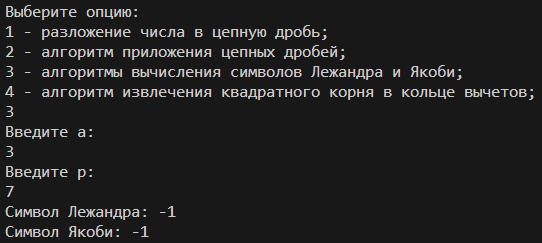
\includegraphics[width=0.8\textwidth]{pic/5.png}
            \caption{Тест алгоритмов вычисления символов Лежандра и Якоби}
        \end{figure}

        \begin{figure}[H]
            \centering
            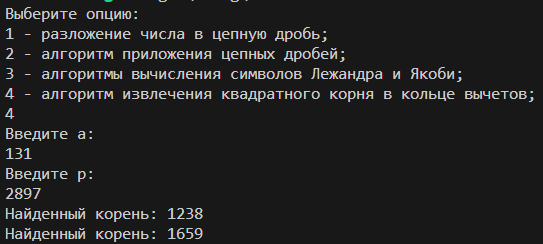
\includegraphics[width=0.8\textwidth]{pic/6.png}
            \caption{Тест алгоритма вычисления квадратного корня в кольце вычетов}
        \end{figure}
\conclusion

    В данной лабораторной работе были рассмотрены теоретические сведения об
    алгоритме разложения чисел в цепную дробь, алгоритмы приложений цепных
    дробей, а также алгоритмы вычисления символов Лежандра и Якоби и извлечения
    квадратного корня в кольце вычетов. На их основе были составлены
    соответствующие алгоритмы. Была произведена оценка сложности созданных
    алгоритмов. Они послужили фундаментом для программной реализации, которая
    впоследствии успешно прошла тестирование, результаты которого были
    прикреплены к отчету вместе с листингом программы, написанной на языке Rust
    с использованием стандартных библиотек языка.

\end{document}
